\documentclass[tikz,border=3pt]{standalone}
\usepackage[T1]{fontenc}
\usepackage{amsmath}
\usepackage{XCharter}
\usepackage[xcharter]{newtxmath}
\usepackage[scaled=.92]{helvet}
\usepackage{pgfplots}
\usetikzlibrary{arrows.meta,positioning,fit,calc,backgrounds,decorations.pathreplacing,patterns}
\usepgfplotslibrary{groupplots,fillbetween}
\pgfplotsset{compat=1.18}
\definecolor{ink}{HTML}{172536}
\definecolor{rgb}{HTML}{3563B8}
\definecolor{event}{HTML}{17857C}
\definecolor{fusion}{HTML}{76529C}
\definecolor{reference}{HTML}{8994A3}
\definecolor{warn}{HTML}{AC5948}
\definecolor{muted}{HTML}{657183}
\definecolor{rule}{HTML}{D9E0E8}
\definecolor{pale}{HTML}{F5F7FA}
\color{ink}
\tikzset{box/.style={rounded corners=2pt,draw=rule,fill=white,align=center,inner sep=4pt,font=\sffamily\fontsize{9}{10.8}\selectfont,minimum height=9mm},rb/.style={box,draw=rgb!50,fill=rgb!5},eb/.style={box,draw=event!50,fill=event!5},fb/.style={box,draw=fusion!55,fill=fusion!5},arrow/.style={-{Latex[length=1.8mm]},line width=.65pt,draw=muted},note/.style={font=\sffamily\fontsize{8.4}{10.2}\selectfont,align=center,text=muted},heading/.style={font=\sffamily\fontsize{10}{12}\selectfont\bfseries,align=left,text=ink}}
\pgfplotsset{paper/.style={width=15.7cm,height=6cm,axis lines*=left,axis line style={rule},tick style={draw=none},tick label style={font=\sffamily\fontsize{8.8}{10.4}\selectfont,text=muted},label style={font=\sffamily\fontsize{9.4}{11}\selectfont,text=ink},title style={font=\sffamily\fontsize{10}{12}\selectfont\bfseries,text=ink},legend style={draw=none,fill=none,font=\sffamily\fontsize{9}{11}\selectfont,cells={anchor=west}},grid=major,grid style={rule!65,line width=.3pt},minor tick num=0,scaled ticks=false,unbounded coords=jump,clip mode=individual}}
\begin{document}

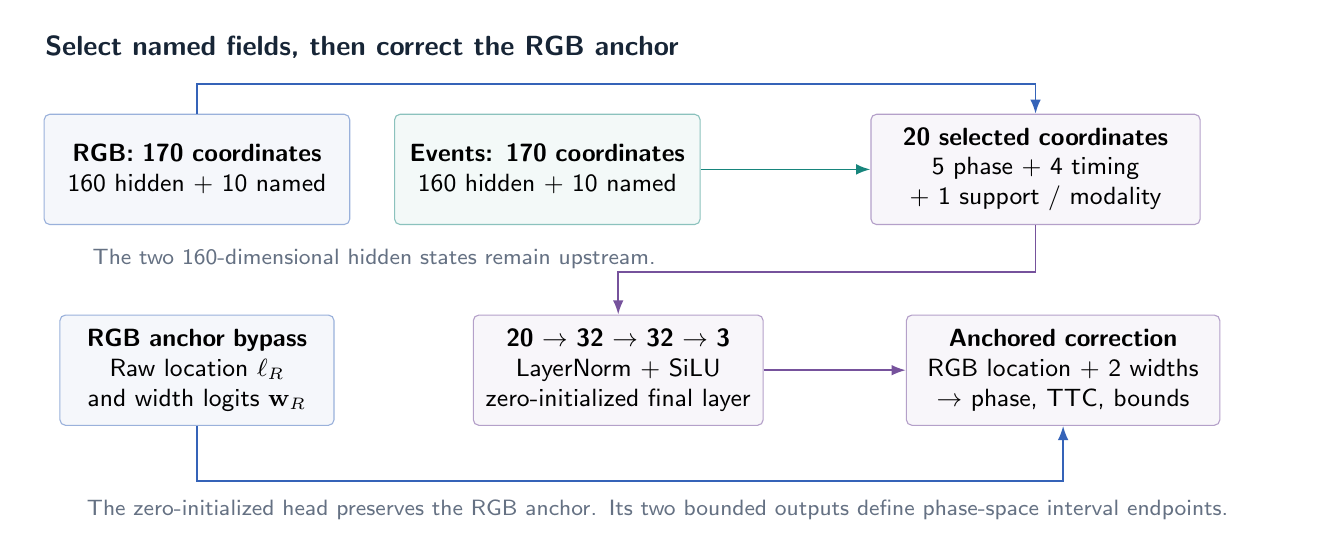
\begin{tikzpicture}[x=1cm,y=1cm]
\path[use as bounding box] (0,-.65) rectangle (16.1,5.6);
\node[heading,anchor=west] at (.1,5.35) {Select named fields, then correct the RGB anchor};
\node[rb,text width=3.6cm,minimum height=14mm] (r) at (2.15,3.8) {\textbf{RGB: 170 coordinates}\\160 hidden + 10 named};
\node[eb,text width=3.6cm,minimum height=14mm] (e) at (6.6,3.8) {\textbf{Events: 170 coordinates}\\160 hidden + 10 named};
\node[fb,text width=3.9cm,minimum height=14mm] (select) at (12.8,3.8) {\textbf{20 selected coordinates}\\5 phase + 4 timing\\+ 1 support / modality};
\draw[arrow,rgb] (r.north)--++(0,.38)-|(select.north);
\draw[arrow,event] (e.east)--(select.west);
\node[note] at (4.4,2.66) {The two 160-dimensional hidden states remain upstream.};
\node[rb,text width=3.2cm,minimum height=14mm] (anchor) at (2.15,1.25) {\textbf{RGB anchor bypass}\\Raw location \(\ell_R\)\\and width logits \(\mathbf w_R\)};
\node[fb,text width=3.4cm,minimum height=14mm] (mlp) at (7.5,1.25) {\textbf{20 \(\to\) 32 \(\to\) 32 \(\to\) 3}\\LayerNorm + SiLU\\zero-initialized final layer};
\node[fb,text width=3.7cm,minimum height=14mm] (o) at (13.15,1.25) {\textbf{Anchored correction}\\RGB location + 2 widths\\\(\to\) phase, TTC, bounds};
\draw[arrow,fusion] (select.south)--++(0,-.6)-|(mlp.north);
\draw[arrow,fusion] (mlp)--(o);
\draw[arrow,rgb] (anchor.south)--++(0,-.7)-|(o.south);
\node[note,text width=15.8cm] at (8,-.52) {The zero-initialized head preserves the RGB anchor. Its two bounded outputs define phase-space interval endpoints.};
\end{tikzpicture}

\end{document}
